%-------------------------------------------------------------------------------------
%	PACKAGES AND THEMES
%-------------------------------------------------------------------------------------
\documentclass{beamer}
\setbeamercovered{transparent}
\setbeamercolor{local structure}{fg=black}
\setbeamertemplate{caption}{\raggedright\insertcaption\par}
\usefonttheme[onlymath]{serif}

\mode<presentation> {
	
	% The Beamer class comes with a number of default slide themes
	% which change the colors and layouts of slides. Below this is a list
	% of all the themes, uncomment each in turn to see what they look like.
	
	%\usetheme{default}
	%\usetheme{AnnArbor}
	%\usetheme{Antibes}
	%\usetheme{Bergen}
	%\usetheme{Berkeley}
	%\usetheme{Berlin}
	%\usetheme{Boadilla}
	\usetheme{CambridgeUS}
	%\usetheme{Copenhagen}
	%\usetheme{Darmstadt}
	%\usetheme{Dresden}
	%\usetheme{Frankfurt}
	%\usetheme{Goettingen}
	%\usetheme{Hannover}
	%\usetheme{Ilmenau}
	%\usetheme{JuanLesPins}
	%\usetheme{Luebeck}
	%\usetheme{Madrid}
	%\usetheme{Malmoe}
	%\usetheme{Marburg}
	%\usetheme{Montpellier}
	%\usetheme{PaloAlto}
	%\usetheme{Pittsburgh}
	%\usetheme{Rochester}
	%\usetheme{Singapore}
	%\usetheme{Szeged}
	%\usetheme{Warsaw}
	
	% As well as themes, the Beamer class has a number of color themes
	% for any slide theme. Uncomment each of these in turn to see how it
	% changes the colors of your current slide theme.
	
	%\usecolortheme{albatross}
	%\usecolortheme{beaver}
	%\usecolortheme{beetle}
	%\usecolortheme{crane}
	%\usecolortheme{dolphin}
	%\usecolortheme{dove}
	%\usecolortheme{fly}
	%\usecolortheme{lily}
	\usecolortheme{orchid}
	%\usecolortheme{rose}
	%\usecolortheme{seagull}
	%\usecolortheme{seahorse}
	%\usecolortheme{whale}
	%\usecolortheme{wolverine}
	
	%\setbeamertemplate{footline} % To remove the footer line in all slides uncomment this line
	%\setbeamertemplate{footline}[page number] % To replace the footer line in all slides with a simple slide count uncomment this line
	
	%\setbeamertemplate{navigation symbols}{} % To remove the navigation symbols from the bottom of all slides uncomment this line
}

\usepackage{graphicx} % Allows including images
\usepackage{booktabs} % Allows the use of \toprule, \midrule and \bottomrule in tables
\usepackage{caption}
\captionsetup{font=scriptsize,labelfont=scriptsize}
\usepackage{amssymb}
\usepackage{bm}
\usepackage[colorinlistoftodos,prependcaption,textsize=small]{todonotes}
%-------------------------------------------------------------------------------------
%	TITLE PAGE
%-------------------------------------------------------------------------------------

\title[Large-Scale Data Analysis Techniques]{A Review on Multi-Label Learning Algorithms} % The short title appears at the bottom of every slide, the full title is only on the title page

\author[Sissy Themeli, Nikiforos Pittaras]{Min-Ling Zhang and Zhi-Hua Zhou} % Your name
\institute[DI-UOA] % Your institution as it will appear on the bottom of every slide, may be shorthand to save space
{
	IEEE Transactions On Knowledge And Data Engineering\\ % Your institution for the title page
	\medskip
}
\date{\today} % Date, can be changed to a custom date

\begin{document}
	
	\begin{frame}
	\titlepage % Print the title page as the first slide
\end{frame}

\begin{frame}
\frametitle{Overview} % Table of contents slide, comment this block out to remove it
\tableofcontents % Throughout your presentation, if you choose to use \section{} and \subsection{} commands, these will automatically be printed on this slide as an overview of your presentation
%\setbeamercolor{section in toc}{fg=black}
%\setbeamercolor{subsection in toc}{fg=black}
\end{frame}

%-------------------------------------------------------------------------------------
%	PRESENTATION SLIDES
%-------------------------------------------------------------------------------------

\section{Introduction} % Sections can be created in order to organize your presentation into discrete blocks, all sections and subsections are automatically printed in the table of contents as an overview of the talk
\subsection{Problem Definition}
%------------------------------------------------
\begin{frame}
\Huge{\centerline{Introduction}}
\end{frame}
%------------------------------------------------
\begin{frame}
\frametitle{\insertsection : \insertsubsection}
Single-label supervised learning
\begin{itemize}
\item Applied to classification
\item Supervised: Dataset $\{ (x_i, y_i)\}, i = 1, \dots N, x \in X, y \in Y$
\item Goal is to learn a model $f: X \rightarrow Y$
\end{itemize}

Multi-label supervised learning
\begin{itemize}
\item Multiple labels per instance: $\{ (x_i, \bm{y}_i)\}, i = 1, \dots N, x \in X, \bm{y} \in \mathbb{P}(Y)$
\item Learn a model $f: X \times Y \rightarrow r$ where $r\in \mathbb{R}$ is the confidence that $y_i$ characterizes $x_i$
\item For classification, assume that $x_i$ belongs to $y_i$ if $r \ge $ $t(x_i)$

\begin{itemize}
\item $t(\cdot)$ can be a predetermined constant function or learned from $X$
\end{itemize}

\end{itemize}
TODO: Include stuff about multi-labeled dataset characterization?
\end{frame}
%------------------------------------------------
\subsection{Related Work}
\begin{frame}
\frametitle{\insertsection : \insertsubsection}
\begin{itemize}
\item Madjarov, Gjorgji, et al. "An extensive experimental comparison of methods for multi-label learning." Pattern Recognition 45.9 (2012): 3084-3104
\item Tsoumakas, Grigorios, and Ioannis Katakis. "Multi-label classification: An overview." International Journal of Data Warehousing and Mining 3.3 (2006)
\item Zhang, Min-Ling, and Kun Zhang. "Multi-label learning by exploiting label dependency." Proceedings of the 16th ACM SIGKDD international conference on Knowledge discovery and data mining. ACM, 2010
\end{itemize}
\end{frame}
%------------------------------------------------
\subsection{Algorithm Strategies}
\begin{frame}
\frametitle{\insertsection : \insertsubsection}
Label search space $\mathbb{S_Y}$ grows exponentially as a function of $|Y|=q$
\begin{itemize}
\item e.g. for $q=20, |\mathbb{S_Y}| = 2 ^ {|\mathbb{P(Y)}|} = 2^{20} \ge 10^6$
\end{itemize}
Solution: integrate in the learning process potential label correlations.
This work examines algorithms grouped in three broad categories:

\begin{enumerate}
\item First-order strategies
\begin{itemize}
\item Transform multi-labeled problem to multiple, single-label problems
\item Ignore label correlations
\item Simple, scalable, suboptimal
\end{itemize}
\item Second-order strategies
\begin{itemize}
\item Consider \emph{pairwise} label relations
\item Good trade-off between generalization performance and scalability
\item Lacking in some real-world applications
\end{itemize}
\item Higher-order strategies
\begin{itemize}
\item Capture more complicated label interdependencies
\item Strong modeling capabilities
\item Computationally demanding, less scalable
\end{itemize}

\end{enumerate}
\end{frame}

%------------------------------------------------
\subsection{Evaluation Metrics}
\begin{frame}
\frametitle{\insertsection : \insertsubsection}
Two categories and perspectives:
\begin{itemize}
\item \emph{Example-based: }Evaluates multi-labelled performance on each example, extrapolate to whole dataset
\begin{itemize}
\item \emph{Classification perspective:}
\begin{itemize}
\item Subset Accuracy, Hamming Loss
\item Precision, Recall, F-measure, F$^\beta$ -measure
\end{itemize}
\item \emph{Ranking perspective:} one-error, coverage, ranking loss, average precision
\end{itemize}
\item \emph{Label-based: }Evaluates performance on each label separately, extrapolate to whole label set
\begin{itemize}
\item Classification perspective: Macro/Micro averaging for single-label example-based, classification-based measures
\item Ranking perspective: Macro/Micro averaging for AUC
\end{itemize}
\end{itemize}
Classifiers should aim to optimize \emph{multiple} metrics
\end{frame}
%------------------------------------------------
\section{Multi-label Learning Algorithms}
%------------------------------------------------
\subsection{Categorization}
%------------------------------------------------
\begin{frame}
\Huge{\centerline{Multi-label Learning Algorithms}}
\end{frame}
%------------------------------------------------
\begin{frame}
\frametitle{\insertsection : \insertsubsection}

Group algorithms in two categories:
\begin{itemize}
\item \emph{Problem Transformation Methods:}

\begin{itemize}
\item Transform the learning problem into other well-established learning scenarios
\item ``Fit data to algorithm'' philosophy
\end{itemize}

\item \emph{Algorithm Adaptation Methods:}
\begin{itemize}
\item Adapt popular learning techniques to deal with multi-label data directly
\item ``Fit algorithm to data'' philosophy
\end{itemize}
\end{itemize}

Include algorithms that:
\begin{itemize}
\item Has broad, unique characteristics
\item Has primitive impact, i.e. leads to a number follow-up related methods
\item Is influential and highly-cited in multi-label learning
\end{itemize}

\end{frame}
%------------------------------------------------
\subsection{Problem Transformation Methods}
%------------------------------------------------
\begin{frame}
\Huge{\centerline{Problem Transformation Methods}}
\end{frame}
%------------------------------------------------
\begin{frame}
\frametitle{\insertsection : \insertsubsection}
\begin{figure}
\begin{center}
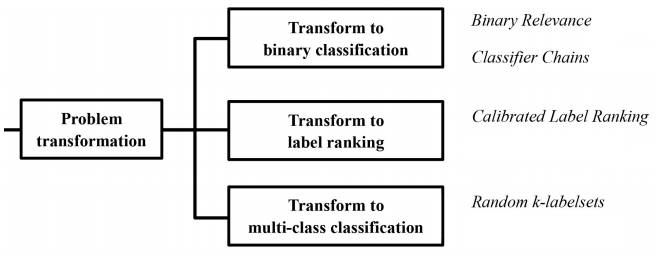
\includegraphics[scale = 0.7]{images/pt.png}
\end{center}
\end{figure}
\end{frame}
%------------------------------------------------
\begin{frame}
\frametitle{Binary Relevance}

\begin{itemize}
\item Decompose multi-label problem to $q$ independent binary classification problems
\item Construct $q$ binary (one-vs-all) training sets (one for each $y_i$)
\item Cross-train each binary classifier $h_i(x)$ on its respective dataset

\item Predict labels of an unseen $x$ by evaluating each classifier $h_i(x)$
\item Output labels where  $h_i(x) > 0$ or $\underset{1 \geq i \geq q}{argmax} \{h_i(x))\}$, if none
\end{itemize}

Pros \& cons:
\begin{itemize}
\item Simple, one-vs-rest scheme, parallelizable
\item Sensitive to class-imbalanced data
\item Ignores label correlations (first-order method)
\end{itemize}

\end{frame}
%------------------------------------------------

\begin{frame}
\frametitle{Classifier chains}
\begin{itemize}
\item A permutation function $f_p$ is used to order $Y$
\item Transform into a \emph{chain} of binary classification problems
\item Enrich representations at each step $j$ by concatenating each $x_i$ with the confidence of the $j$-th classifier
\item Predict relevant labels for unknown instances by iteratively traversing the classifier chain
\end{itemize}

Pros \& cons:
\begin{itemize}
\item Higher-order method: exploitation of label correlations, but in a random manner
\item Highly sensitive to $f_p$. Ensemble schemes attempt to overcome it.
\item Iterative operation prevents parallel implementation
\end{itemize}
\end{frame}
%------------------------------------------------

\begin{frame}
\frametitle{Calibrated Label Ranking}
\begin{itemize}
\item Transform into a label pairwise comparison ranking problem
\item For $q$ labels, generate $q(q-1)/2$ binary classifiers by pairwise comparison
\item Construct training sets $D_{jk} : \{x_i | y_j \in Y_i \oplus y_k \in Y_i\}$
\item For an unknown instance, all classifiers' votes are aggregated and ranked
\item A virtual label $y_v$ serves as the artificial splitting point between relevant and irrelevant labels
\end{itemize}
Pros \& cons:
\begin{itemize}
\item Second-order approach algorithm. One-vs-one scheme.
\item Smooths out the class-imbalance problem
\item Number of classifiers s quadratic to $|Y|$ (compared to linear for BR)
\begin{itemize}
\item Pruning methods to reduce the search space
\end{itemize}
\end{itemize}
\end{frame}
%------------------------------------------------
\begin{frame}
\frametitle{Random k-Labelsets}
\begin{itemize}
\item Decompose to an ensemble of multi-class classification problems
\item Each component targets a random subset of $Y$, classified with Label Powerset (LP) techniques:
\begin{itemize}
\item Transform to single-label data by treating each distinct labelset as a new class
\item Each example is reassigned with the mapped single-label participating in multi-class classifier induction
\item For unknown $x$, counts the maximum and actual number of votes
\item Label set is relevant when the number of votes exceeds half of the max
\end{itemize}
\end{itemize}
Pros \& cons:
\begin{itemize}
\item High-order approach algorithm
\item Data-sensitive: Cannot generalize to labelsets not in the training set, too few examples for some labelsets
\item Large $Y$ implies high training complexity.
\item Improve by invoking an ensemble on random k-sized labelsets
\end{itemize}
\end{frame}
%------------------------------------------------
\subsection{Alogrithm Adaptation Methods}
%------------------------------------------------
\begin{frame}
\Huge{\centerline{Algorithm Adaptation Methods}}
\end{frame}
%------------------------------------------------
\begin{frame}
\frametitle{\insertsection : \insertsubsection}
\begin{figure}
\begin{center}
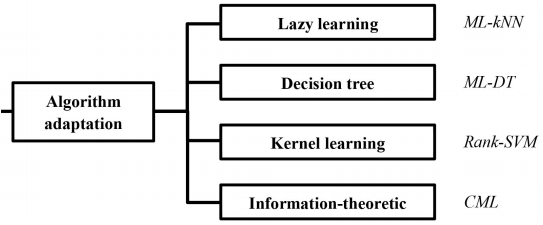
\includegraphics[scale = 0.75]{images/aa.png}
\end{center}
\end{figure}
\end{frame}
%------------------------------------------------
\begin{frame}
\frametitle{Multi-Label k-Nearest Neighbour}
\begin{itemize}
\item First-order approach algorithm, adapting knn techniques
\item Compares the MAP probabilities: $P(K|C_j), K \in \{H_j, \neg H_j\}$
\item Priors $P(K)$ computed by smoothed frequency estimation in the training data
\item Likelihoods $P(C_j|K)$ are computed as a function of:
\begin{itemize}
\item $\kappa(r)$, the number of examples labelled $y_j$ with $r$ neighbours labelled $y_j$
\item $\overset{\sim}{\kappa}(r)$, the number of examples not labelled $y_j$ with $r$ neighbours labelled $y_j$
\end{itemize}
\end{itemize}

Pros \& cons:
\begin{itemize}
\item First-order approach, Bayesian and Lazy reasoning
\item Decision boundary can be modified on-line via new instances
\item Class imbalance can be overcome by calculating priors
\item Extensions proposed for label correlation exploitations
\end{itemize}


\end{frame}
%------------------------------------------------
\begin{frame}
\frametitle{Multi-label Decision Tree}
\begin{itemize}
\item Multi-label entropy is used to build a decision tree recursively
\item Split position is such that the information gain criterion is maximized
\item Dataset $T$ is split on the $l$-th feature valued $\theta$ to branches ($T^-$ \& $T^+$), where $ x_{il} \leq \theta, x_i \in T^-$ and $ x_{il} > \theta, x_i \in T^+$
\item Recurse on subtrees until a stopping criterion is met (e.g. child size)
\item Single-label entropy is computed by considering labelsets as new classes
\item Assumes independence among labels to ensure low computational cost
\item Unseen instances are assigned the label of the majority of members of the leaf they arrive
\end{itemize}
Pros \& cons:
\begin{itemize}
\item First-order algorithm, highly efficient
\item Assumes label independence
\item Pruning and ensemble strategies proposed
\end{itemize}
\end{frame}
%------------------------------------------------
\begin{frame}
\frametitle{Ranking Support Vector Machine}
\begin{itemize}
\item $q$ linear classifiers, optimized to minimize the empirical ranking loss
\item For each relevant-nonrelevant label pair $(y_j,y_k) \in Y_j \times \bar Y$ their decision boundary is marked by $\left<w_j,w_k\right> + b_j - b_k=0$
\item Retrieves a ranked label pairs list for each unseen instance
\item Non-linearity achievable through feature mapping and the kernel trick
\item Convex quadratic programming problem, solved by any QP solver
\end{itemize}
Pros \& cons:
\begin{itemize}
\item Second-order approach, maximum margin strategy
\item Extensible by kernel learning, kernel selection can be overcome by MKL techniques
\item Adaptable learning by selecting an appropriate loss function
\end{itemize}

\end{frame}
%------------------------------------------------
\begin{frame}
\frametitle{Collective Multi-Label Classifier}
\begin{itemize}
\item Labels encoded as binary random vectors into a joint pdf
\item Label correlations encoded into the joint pdf as constraints
\item Model via the maximum information entropy criterion: $H_p(x, y)$, subject to constraints $\mathbb{E_p}[f_k(x,y)] = F_k$, where $F_k$ are estimated from the training set
\item Objective arrived by Lagrange multipliers, solvable by any constraint optimization solver
\item Unseen instances labelled with $Y = \underset{y}{\text{argmax }} P(y | x)$
\end{itemize}
Pros \& cons:
\begin{itemize}
\item Second-order approach. All label pairs considered, not just relevant-irrelevant ones.
\item Intractable $\text{argmax}$ operation for a large label space without pruning.
\end{itemize}
\end{frame}
%------------------------------------------------
\begin{frame}
\frametitle{\insertsection : Summary}
\begin{figure}
\begin{center}
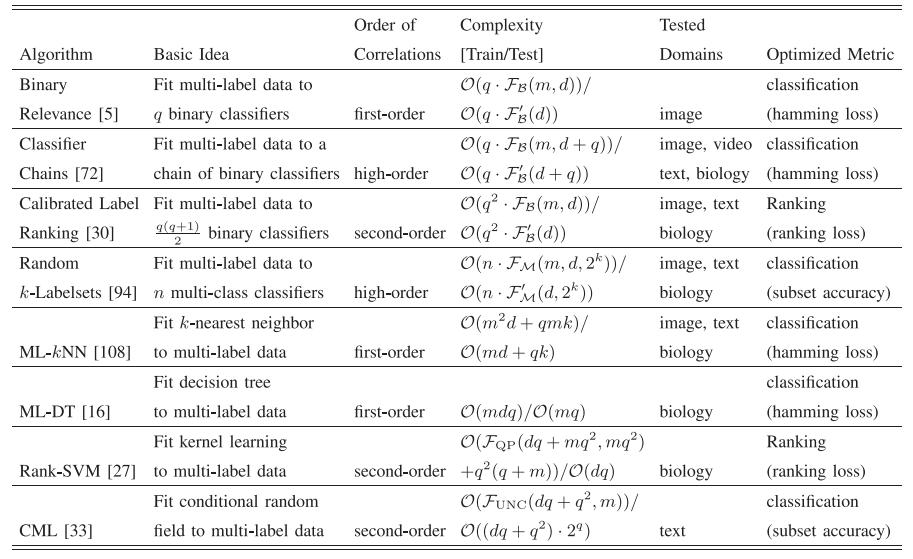
\includegraphics[scale = 0.45]{images/summary.png}
\caption{Summary of Representative Multi-Label Learning Algorithms}
\end{center}
\end{figure}
\end{frame}
%------------------------------------------------
\section{Related Learning Settings}
%------------------------------------------------
\begin{frame}
\frametitle{\insertsection}
\begin{itemize}
\item Multi-instance learning
\begin{itemize}
\item Each ML example described by a bag of instances while associated with a single/binary label
\item Models the object’s complex semantics in input space, rather than its output
\end{itemize}
\item Ordinal classification
\begin{itemize}
\item Model class co-relevance in a (vague) graded membership vector
\item Transform ML problem to a set of ordinal set of problems
\end{itemize}
\item Multi-task learning
\begin{itemize}
\item Multiple tasks trained in parallel, sharing information
\item Knowledge from related tasks used as an inductive bias to improve generalization
\item Shared or different feature space, small task workload
\end{itemize}
\item Data streams classification
\begin{itemize}
\item Real-world objects are generated online and processed in  real-time
\item Concept drift problem
\end{itemize}
\end{itemize}
\end{frame}

%------------------------------------------------
\section{Conclusion}
%------------------------------------------------
\begin{frame}
\Huge{\centerline{Conclusion}}
\end{frame}
%------------------------------------------------
\begin{frame}
\frametitle{\insertsection : Online resources}
\begin{figure}
\begin{center}
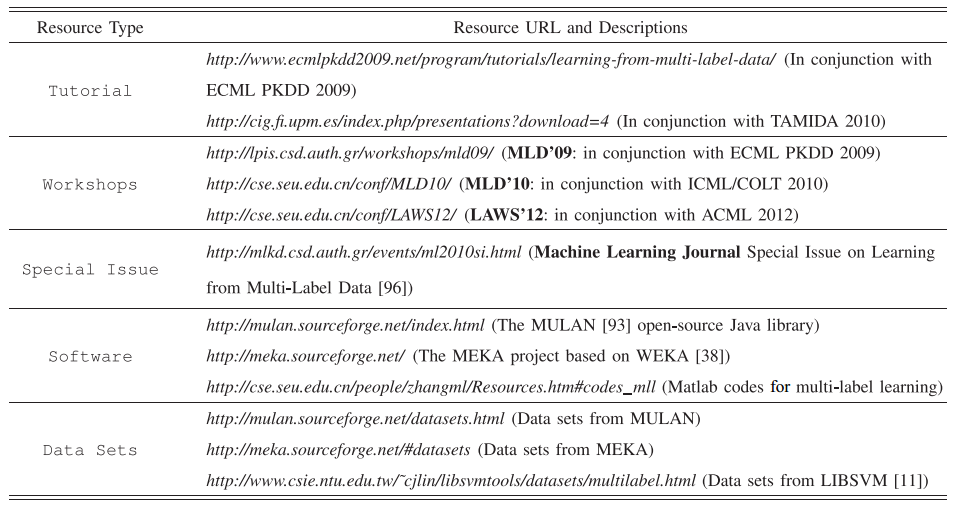
\includegraphics[scale = 0.47]{images/online.png}
\caption{Online Resources for Multi-Label Learning}
\end{center}
\end{figure}
\end{frame}
%------------------------------------------------
\begin{frame}
\frametitle{\insertsection}
Summary:
\begin{itemize}
\item Multi-label learning problem definition
\item Multi-label learning representative algorithms
\item Related learning settings
\end{itemize}

Future goals:
\begin{itemize}
\item Holy grail: Formal characterization on the underlying concept / mechanism on the appropriate usage of label correlations, especially on large output spaces
\item Thorough experimental comparative study to discover pros and cons of different multi-label learning algorithms
\end{itemize}
\end{frame}

%------------------------------------------------
\section{The end}
\begin{frame}
\Huge{\centerline{Thank you}}
\Huge{\centerline{Questions?}}
\end{frame}
%------------------------------------------------
\end{document}
